\section{Appareil à raclette (5 points)}

Lorsqu'elle est traversée par un courant électrique, une résistance produit de la chaleur, c'est l'effet Joule.
La résistance de l'appareil à raclette de Martin ne fonctionne plus ! Dans son garage, il trouve deux résistances qui pourraient peut-être convenir pour la remplacer. 
Les documents ci-dessous présentent le résultats de la mesure à l'ohmmètre des deux résistances et le descriptif technique de l'appareil à raclette.
%\begin{multicols}{2}
	\begin{center}
		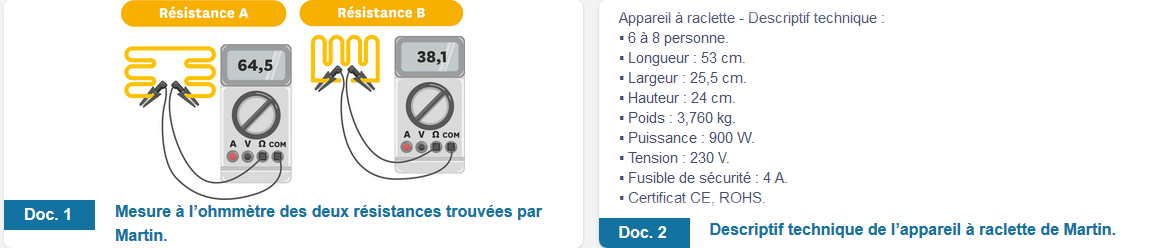
\includegraphics[scale=0.7]{img/docs}
		%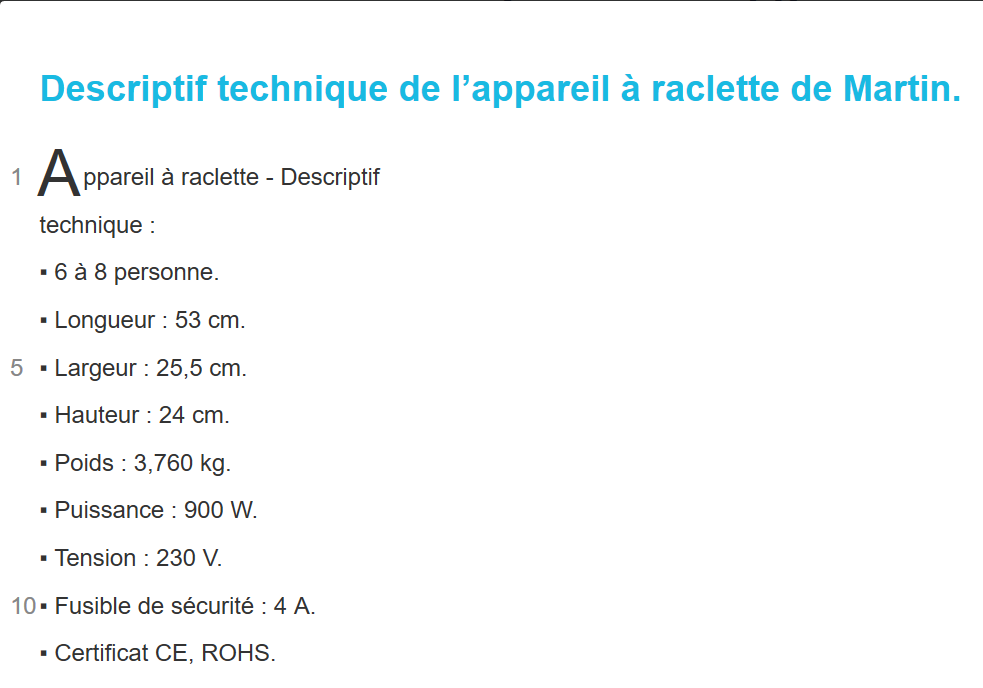
\includegraphics[scale=0.5]{img/doc2}
	\end{center}
%\end{multicols}

\begin{questions}
	\question[1] Quelles informations du descriptif technique permettront de savoir quelle sera la résistance appropriée ?
	\begin{solution}
		Sur le descriptif technique, le tension et nominale et la valeur du fusible permettront d'identifier la résistance appropriée.
	\end{solution}
	
	\question[1\half] Quelle valeur de résistance correspond à l'intensité maximale ?
	\begin{solution}
		L'intensité maximale supportée par l'appareil à raclette correspond à la valeur du fusible, c'est à dire 4 $A$. D'après la loi d'Ohm, on a :
		
		\begin{eqnarray*}
			U &=& R \times I \\
			R &=& \frac{U}{I} \\
			R &=& \frac{230}{4} \\
			R &=& \num{57.5}
		\end{eqnarray*}
	
	Donc l'intensité maximale correspond à une résistance de \num{57.5} $\Omega$.
	\end{solution}
	
	\question[1\half] Quelle résistance devra choisir Martin ?
	\begin{solution}
		Il devra choisir une valeur de résistance plus faible que la résistance maximale, c'est à dire la résistance B.
	\end{solution}
	
	\question[1] Que se passerait-il s'il choisissait l'autre ?
	\begin{solution}
		S'il choisissait l'autre, il dépasserait l'intensité maximale donc le fusible grillerait et ouvrirait le circuit pour éviter une surintensité.
	\end{solution}
\end{questions}